\documentclass{standalone}
\usepackage{graphicx}
\usepackage{tikz}
\usetikzlibrary{shapes.geometric, arrows}

\tikzset{
    to/.style     = {->, line width=0.4mm},
    line/.style   = {line width=0.6mm, draw=blue},
    darrow/.style = {<-, line width=0.6mm, draw=blue},
    box/.style    = {draw, rectangle, rounded corners, minimum height = 2.5cm, text centered, text width=4.5cm, fill=white, font=\Huge\sffamily}
}

\pgfmathsetmacro{\ex}{0.70}
\pgfmathsetmacro{\ey}{0.60}

\begin{document}
\begin{tikzpicture}
	\node[anchor=south west,inner sep=0] (image) at (0,0,0) {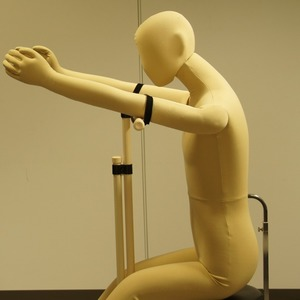
\includegraphics[width=\linewidth]{up}};
	\begin{scope}[x={(image.south east)},y={(image.north west)}]
		\iffalse
			%% Next four lines helps to locate the point needed by forming a grid
			\draw[help lines,xstep=.1,ystep=.1] (0,0) grid (1,1);
			\draw[help lines,xstep=.05,ystep=.05] (0,0) grid (1,1);
			\foreach \x in {0,1,...,9} {\node[anchor=north] at (\x/10,0) {0.\x}; }
			\foreach \y in {0,1,...,9} {\node[anchor=east] at (0,\y/10) {0.\y};}
		\fi
		\begin{scope}[x={(image.south east)},y={(image.north west)}]
			\draw[line] (0.10,0.60) -- (\ex,\ey);
			\draw[line] (0.10,0.76) -- (\ex,\ey);
			\draw[to, draw=blue](\ex,\ey) ++(180:.35) arc (180:165.5:.35);
			\draw[to](0.22,0.45) node[box]{Angle of Inclination} to [out=90,in=180] (0.35,0.65);
		\end{scope}
	\end{scope}
\end{tikzpicture}
\end{document}
